This section is devoted to validate our proposal named as ``Case 5''.
%
The WFG \cite{Joel:WFG}, DTLZ \cite{Joel:DTLZ_2} and UF \cite{zhang2009performance} test problems have been used for our purpose.
%
Our experimental validation includes the Differential Evolution based variants DEMO such strategy is explained in \cite{tuvsar2007differential}.
%
Given that all of them are stochastic algorithms, each execution was repeated $35$ times with different seeds.
%
The common configuration in all of them was the following: the stopping criterion was set to $25,000$ generations, the population size was fixed to 100, the WFG test problems were configured with two and three objectives, setting 24 parameters, where 20 of them are distance parameters and 4 are position parameters.
%
Specifically, in the DTLZ test instances, the number of decision variables is set to $n=M+r-1$, where $r=\{5, 10, 20\}$ for DTLZ1, DTLZ2 to DTLZ6 and DTLZ7 respectively, as is suggested by the authors \cite{Joel:DTLZ_2}.  
% 
The UF benchmark is composed of ten test instances, where the first seven are of two objectives and the rest with three objectives, the number of decision variables is assigned to $n=10$.
%
In general, the crossover and mutation operators are SBX and polynomial respectively, with a crossover probability of 0.9 and mutation probability of $1/n$, also the crossover and mutation distribution indexes were assigned to 20 and 50 respectively.
%
The extra parametrization of each algorithm is as follows:
\begin{itemize}
\item \textbf{DE-Variants}: CR = 0.3 and F = 0.5.
\item \textbf{SMS-EMOA}: offset = 100.
\item \textbf{MOEA/D}: size of neighborhood = 10, max updates by sub-problem (nr) = 2 and $\delta = 0.9$.
\end{itemize}
%
Our experimental analysis has been performed in base of the Normalized HV and IGD+.
%
The reference points implemented in the hypervolume indicator are showed in the Table \ref{tab:ReferencePoints} as used in \cite{Joel:Kuhn_Munkres, Joel:OperatorAHX}.


In order to statistically compare the hypervolume results, a similar guideline than the proposed in \cite{Joel:StatisticalTest} was used. 
%
First a Shapiro-Wilk test was performed to check whatever or not the values of the results followed a Gaussian distribution. 
%
If, so, the Levene test was used to check for the homogeneity of the variances. 
%
If samples had equal variance, an ANOVA test was done; if not, a Welch test was performed. 
%
For non-Gaussian distributions, the nonparametric Kruskal-Wallis test was used to test whether samples are drawn from the same distribution. 
%
An algorithm $X$ is said to win algorithm $Y$ when the differences between them are statistically significant, if the mean and median obtained by $X$ are higher than the mean and median achieved by $Y$.
%

In addition, pair-wise statistical tests with HV and IGD+ were performed (Table \ref{tab:statistical_Tests}).
%
For each instance, the column ``$\uparrow$'' reports the number of comparisons where the statistical tests confirmed the superiority of the MOEA listed in the corresponding group, whereas the column ``$\downarrow$'' reports the number of cases where it was inferior and ``$\longleftrightarrow$'' indicates that are not significantly different and is considered as a tie.
%%


Based in the statistical tests\footnote{DE is not considered in the statistical tests.} (Table \ref{tab:statistical_Tests}), generally speaking our proposal (Case 5) has the best scores.
%
Our proposal is outperformed by the Case 4 considering three objectives by the NSGA-II, this might occurs due that this MOEA applies a binary tournament selection where is considered the dominance concept, thus some level of diversity is maintained, therefore in some problems some optimal regions are reached, and with other problems the solutions could be far from the Pareto front.
%
Although that in average the metrics are similar between the Case 4 and our proposal with three objectives, the average difference with the best indicates that our proposal is the closest to the best since that it shows in the ``Average Best Difference'' IGD+ with $0.020$ against the Case 4 with $0.023$.
%
Also, inspecting the statistical test, the Case 4 has more lost than our proposal $10$ against $9$ and $15$ against $9$ of the HV and IGD+ respectively.
%
However, the MOEA/D and SMS-EMOA which are more elitist algorithms and do not consider the dominance concept at all, are not affected in this sense.
%
Anyway, our proposal and the Case 3 reports significantly better results that the normal SBX (Case 1), in fact this could evidence that variate the distribution index among the execution has an important effect.


In order to better understand the behavior of our proposal, the Tables \ref{tab:Metrics_2} and \ref{tab:Metrics_3} shows a summary average of Normalized HV and IGD+ considering all the instances\footnote{The detailed results can be consulted in the web page https:\//\//github.com\//joelchaconcastillo\//SBX\_CEC2018.}.
%
Also is counted the number of instances which attain the best results labeled by ``Best Counts''.
%
Additionally, the average of difference with the best result is showed, this aims to provide a metric which indicates the difference with the best result attained in each problem.
%
Although that DE improves our proposal with two objectives, in the Table \ref{tab:Metrics_2}  is showed that our proposal provides near results than the bests.
%

On the other hand our proposal provides the best results considering three objectives, it is interesting remark that the performance of DE is seriously deteriorated according increases the number of objectives. 
%
Despite the fact that DE variants have high ``Best Count'' values, in average it is improved by the Case 4 and Case 5, this might occurs because DE is directly influence by the parameters (CR and FR), therefore in some instances the DE variants attains the best results, and in other instances the solutions are far from the Pareto front.
%

On the other hand, our proposal shows a robust behavior in the state-of-the-art MOEAs, in fact the ``Average Best Difference'' is low both with two objectives and three objectives that confirms the stability and superiority of our proposal.
%
\begin{table}[t]
\centering
\scriptsize
\caption{References points for the HV indicator}
\label{tab:ReferencePoints}
\begin{tabular}{cc}
\hline
\textbf{Instances} & \textbf{Reference Point} \\ \hline
WFG1-WFG9 & $[2.1, ...,2m+0.1]$ \\
DTLZ 1, 2, 4 & $[1.1, ..., 1.1]$ \\
DTLZ 3, 5, 6 & $[3, ..., 3]$ \\
DTLZ7 & $[1.1, ..., 1.1, 2m]$ \\
UF 1-10 & $[2, ..., 2]$ \\ \hline
\end{tabular}
\end{table}
% % Please add the following required packages to your document preamble:
% % \usepackage{multirow}
% % \usepackage{graphicx}
% \begin{table*}[]
% \centering
% \caption{Statistical Information of Metrics}
% \label{my-label}
% \resizebox{\textwidth}{!}{%
% \begin{tabular}{|l|c|c|c|c|c|c|c|c|c|c|c|c|c|c|c|c|c|c|c|}
% \hline
% \multicolumn{2}{|l|}{\multirow{2}{*}{}} & \multicolumn{6}{c|}{NSGA-II} & \multicolumn{6}{c|}{MOEA/D} & \multicolumn{6}{c|}{SMS-EMOA} \\ \cline{3-20} 
% \multicolumn{2}{|l|}{} & 1 & 2 & 3 & 4 & 5 & 6 & 1 & 2 & 3 & 4 & 5 & 6 & 1 & 2 & 3 & 4 & 5 & 6 \\ \hline
% \multirow{6}{*}{2 Objectives} & Average HV & 0.88 & 0.90 & 0.90 & 0.91 & 0.93 & \textbf{0.94} & 0.87 & 0.87 & 0.87 & 0.90 & \textbf{0.91} & \textbf{0.91} & 0.88 & 0.89 & 0.87 & 0.91 & 0.92 & \textbf{0.93} \\ \cline{2-20} 
%  & Best Counts HV & 2 & 1 & 0 & 1 & 8 & \textbf{11} & 2 & 0 & 2 & 2 & 8 & \textbf{9} & 0 & 1 & 1 & 5 & 6 & \textbf{10} \\ \cline{2-20} 
%  & \multicolumn{1}{l|}{Average Best Difference HV} & \multicolumn{1}{l|}{0.068} & \multicolumn{1}{l|}{0.057} & \multicolumn{1}{l|}{0.053} & \multicolumn{1}{l|}{0.039} & \multicolumn{1}{l|}{0.019} & \multicolumn{1}{l|}{\textbf{0.017}} & \multicolumn{1}{l|}{0.053} & \multicolumn{1}{l|}{0.048} & \multicolumn{1}{l|}{0.049} & \multicolumn{1}{l|}{0.024} & \multicolumn{1}{l|}{\textbf{0.013}} & \multicolumn{1}{l|}{0.014} & \multicolumn{1}{l|}{0.074} & \multicolumn{1}{l|}{0.064} & \multicolumn{1}{l|}{0.081} & \multicolumn{1}{l|}{0.045} & \multicolumn{1}{l|}{0.028} & \multicolumn{1}{l|}{\textbf{0.019}} \\ \cline{2-20} 
%  & Average IGD+ & 0.12 & 0.09 & 0.11 & 0.07 & 0.06 & \textbf{0.05} & 0.14 & 0.12 & 0.14 & 0.09 & 0.08 & \textbf{0.07} & 0.13 & 0.11 & 0.14 & 0.08 & 0.07 & \textbf{0.05} \\ \cline{2-20} 
%  & Best Counts IGD+ & 2 & 1 & 1 & 1 & 8 & \textbf{10} & 3 & 0 & 2 & 3 & 6 & \textbf{9} & 0 & 2 & 0 & 3 & \textbf{9} & \textbf{9} \\ \cline{2-20} 
%  & \multicolumn{1}{l|}{Average Best Difference IGD+} & \multicolumn{1}{l|}{0.086} & \multicolumn{1}{l|}{0.052} & \multicolumn{1}{l|}{0.077} & \multicolumn{1}{l|}{0.035} & \multicolumn{1}{l|}{0.021} & \multicolumn{1}{l|}{\textbf{0.016}} & \multicolumn{1}{l|}{0.075} & \multicolumn{1}{l|}{0.059} & \multicolumn{1}{l|}{0.072} & \multicolumn{1}{l|}{0.025} & \multicolumn{1}{l|}{0.019} & \multicolumn{1}{l|}{\textbf{0.008}} & \multicolumn{1}{l|}{0.093} & \multicolumn{1}{l|}{0.071} & \multicolumn{1}{l|}{0.101} & \multicolumn{1}{l|}{0.038} & \multicolumn{1}{l|}{0.030} & \multicolumn{1}{l|}{\textbf{0.017}} \\ \hline
% \multirow{6}{*}{3 Objectives} & Average HV & \textbf{0.87} & 0.84 & \textbf{0.87} & \textbf{0.87} & \textbf{0.87} & 0.85 & 0.84 & 0.84 & 0.84 & \textbf{0.86} & \textbf{0.86} & 0.85 & 0.90 & 0.89 & 0.88 & \textbf{0.91} & \textbf{0.91} & \textbf{0.91} \\ \cline{2-20} 
%  & Best Counts HV & 1 & 2 & 1 & 4 & 4 & \textbf{7} & 1 & 2 & 1 & 2 & 5 & \textbf{8} & 3 & 2 & 0 & 2 & 5 & \textbf{7} \\ \cline{2-20} 
%  & \multicolumn{1}{l|}{Average Best Difference HV} & \multicolumn{1}{l|}{0.019} & \multicolumn{1}{l|}{0.047} & \multicolumn{1}{l|}{0.020} & \multicolumn{1}{l|}{\textbf{0.014}} & \multicolumn{1}{l|}{\textbf{0.014}} & \multicolumn{1}{l|}{0.032} & \multicolumn{1}{l|}{0.036} & \multicolumn{1}{l|}{0.041} & \multicolumn{1}{l|}{0.038} & \multicolumn{1}{l|}{0.016} & \multicolumn{1}{l|}{\textbf{0.013}} & \multicolumn{1}{l|}{0.027} & \multicolumn{1}{l|}{0.038} & \multicolumn{1}{l|}{0.038} & \multicolumn{1}{l|}{0.049} & \multicolumn{1}{l|}{\textbf{0.019}} & \multicolumn{1}{l|}{0.027} & \multicolumn{1}{l|}{\textbf{0.019}} \\ \cline{2-20} 
%  & Average IGD+ & 0.13 & 0.16 & 0.13 & \textbf{0.12} & \textbf{0.12} & 0.13 & 0.15 & 0.14 & 0.15 & \textbf{0.11} & \textbf{0.11} & 0.13 & 0.11 & 0.11 & 0.13 & \textbf{0.09} & \textbf{0.09} & 0.13 \\ \cline{2-20} 
%  & Best Counts IGD+ & 0 & 2 & 2 & 4 & 3 & \textbf{8} & 2 & 2 & 0 & 2 & 4 & \textbf{9} & 1 & 3 & 0 & 3 & 5 & \textbf{7} \\ \cline{2-20} 
%  & \multicolumn{1}{l|}{Average Best Difference IGD+} & \multicolumn{1}{l|}{0.029} & \multicolumn{1}{l|}{0.061} & \multicolumn{1}{l|}{0.027} & \multicolumn{1}{l|}{0.023} & \multicolumn{1}{l|}{\textbf{0.020}} & \multicolumn{1}{l|}{0.032} & \multicolumn{1}{l|}{0.053} & \multicolumn{1}{l|}{0.048} & \multicolumn{1}{l|}{0.053} & \multicolumn{1}{l|}{\textbf{0.015}} & \multicolumn{1}{l|}{\textbf{0.015}} & \multicolumn{1}{l|}{0.030} & \multicolumn{1}{l|}{0.047} & \multicolumn{1}{l|}{0.040} & \multicolumn{1}{l|}{0.062} & \multicolumn{1}{l|}{\textbf{0.020}} & \multicolumn{1}{l|}{0.024} & \multicolumn{1}{l|}{0.069} \\ \hline
% \end{tabular}%
% }
% \end{table*}


% \begin{figure}[!t]
% \centering
% \includegraphics[scale=0.25,angle=-90]{img/bar_HV_2obj.eps}
% \caption{Average of normalized hypervolume considering all the instances and two objective.}
% \label{fig_sim}
% \end{figure}
% \begin{figure}[]
% \centering
% \includegraphics[scale=0.25,angle=-90]{img/bar_IGD_2obj.eps}
% \caption{Average of Inverted Genralized Distance Plus (IGD+) considering all the instances and two objective.}
% \label{fig_sim}
% \end{figure}

% \begin{figure}[!t]
% \centering
% \includegraphics[scale=0.25,angle=-90]{img/bar_HV_3obj.eps}
% \caption{Average of normalized hypervolume considering all the instances and three objective.}
% \label{fig_sim}
% \end{figure}
% \begin{figure}[]
% \centering
% \includegraphics[scale=0.25,angle=-90]{img/bar_IGD_3obj.eps}
% \caption{Average of Inverted Genralized Distance Plus (IGD+) considering all the instances and three objective.}
% \label{fig_sim}
% \end{figure}
